\documentclass[11pt]{article}
\usepackage{natbib,mybigpackage}
\usepackage{algorithm}
%\usepackage{program}
%\usepackage{algpseudocode}
\usepackage{algorithmic}
\usepackage{listings}


\def\xbf{\mathbf{x}}
\def\zbf{\mathbf{z}}
\def\xibf{\mathbf{\xi}}
\title{MA 226 - Assignment Report 3}
\author{Ayush Sharma\\150123046}
\begin{document}
\titlepage
\newpage

\begin{enumerate}
\item[Q 1]  Implement the linear congruence generator
$x_{i+1} = a x_i ~~ \mbox{mod} ~~ m$
to generate a sequence $x_i$ and hence uniform random numbers $u_i$ .
Make use of the following set of values of a and m:
(a) $a = 16807$ and $m = 2^{31} - 1$.
(b) $a = 40692$ and $m = 2147483399$.
(b) $a = 40014$ and $m = 2147483563$.

Group the values into equidistant ranges for the values of $u_{i}$. Tabulate the proportions and draw a bar diagram for the above. What do you observe ? Do it for 1000, 10000 and 100000 values.

For part (a) do the following: Plot the values $(u_{i}, u_{i+1})$ on a unit square. Now, zoom into the range $u_{i}$ $\epsilon$ [0, 0.001]. What are your observations ?
\end{enumerate}

\noindent{Code for C}

\begin{lstlisting}
#include <stdio.h>
#include <stdlib.h>
#include <math.h>

void plot(unsigned long long int a, unsigned long long int m, unsigned long long int x0, unsigned long long int v0){
	unsigned long long int x = x0, v = 0;
	float u, u1;
	u1 = (x/(float)m);
	do{
		u = u1;
		x = (((a * x) + 0) % m);
		u1 = (x/(float)m);
		printf("(%g,%g)\t", u, u1);
		v++;
	}while(x != x0 && v <= v0);
	printf("\n");
}

void gen(unsigned long long int a, unsigned long long int m, unsigned long long int x0, unsigned long long int * f, unsigned long long int v0){
	unsigned long long int x = x0, v = 0; int i = 0;
	do{
		x = (((a * x) + 0) % m);
		i = ((x/(float)m)/0.05);
		if (i == 20) {i--;}
		*(f + i) += 1;
		v++;
	}while(x != x0 && v <= v0);

//Printing the frequency table:
	for(int j = 0; j < 20; j++){
		printf("\t\t%.2f-%.2f\t:\t%llu\n", (j/(float)20), ((j+1)/(float)20), *(f+j));
	}
}

void main(){
	unsigned long long int x0, f[3][3][20] = {0};

//Frequency Distributuions:
	printf("Frequency Distributions :");
//Part (a)
	printf("\nFor a = 16807, m = 2^(31) - 1, and x0 = 1 :");
	printf("\n\t#For 1000 values ::\n");
	gen(16807, (pow(2,31) - 1), 1, *(*(f+0)+0), 1000);

	printf("\n\t#For 10000 values ::\n");
	gen(16807, (pow(2,31) - 1), 1, *(*(f+0)+1), 10000);

	printf("\n\t#For 100000 values ::\n");
	gen(16807, (pow(2,31) - 1), 1, *(*(f+0)+2), 100000);

//Part (b)
	printf("\n\nFor a = 40692, m = 214748339, and x0 = 1 :");
	printf("\n\t#For 1000 values ::\n");
	gen(40692, 2147483399, 1, *(*(f+1)+0), 1000);

	printf("\n\t#For 10000 values ::\n");
	gen(40692, 2147483399, 1, *(*(f+1)+1), 10000);

	printf("\n\t#For 100000 values ::\n");
	gen(40692, 2147483399, 1, *(*(f+1)+2), 100000);

//Part (c)
	printf("\n\nFor a = 40014, m = 214748356, and x0 = 1 :");
	printf("\n\t#For 1000 values ::\n");
	gen(40014, 2147483563, 1, *(*(f+2)+0), 1000);

	printf("\n\t#For 10000 values ::\n");
	gen(40014, 2147483563, 1, *(*(f+2)+1), 10000);

	printf("\n\t#For 100000 values ::\n");
	gen(40014, 2147483563, 1, *(*(f+2)+2), 100000);

//Printing (u_i, u_i+1)
	printf("Plot data :");
	printf("\nFor a = 16807, m = 2^(31) - 1, and x0 = 1 :\n\tThe values (u_i, u_i+1) are :: ");
	plot(16807, (pow(2,31) - 1), 1, 100000);
}
\end{lstlisting}
\newpage
\noindent{\textbf{Result}:}

The histograms can be shown as :

\begin{figure}[H]
  \centering
  \captionsetup{justification=centering}
  \subfloat[$\xi_{1}$]{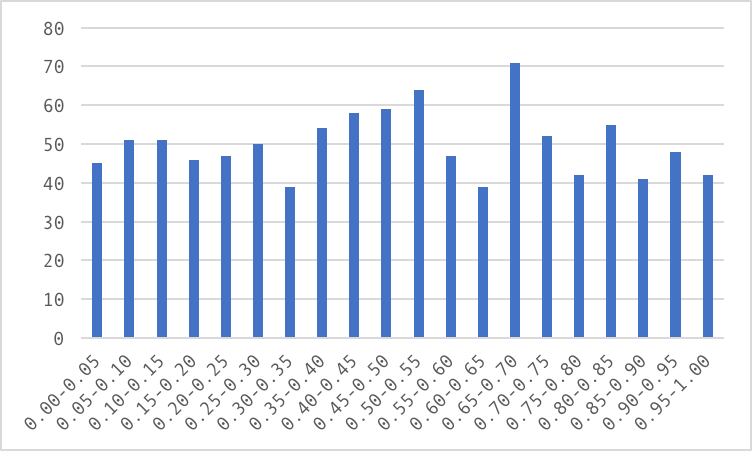
\includegraphics[width=0.5\textwidth]{1000a.png}}\hspace{10mm}
  \subfloat[$\xi_{2}$]{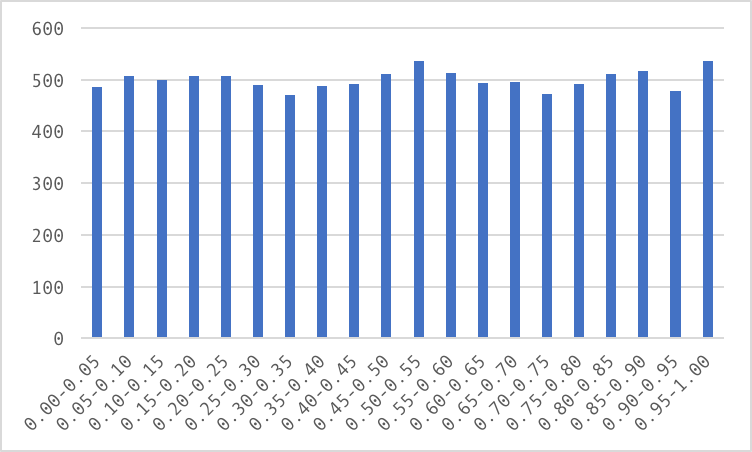
\includegraphics[width=0.5\textwidth]{10000a.png}}\\
  \subfloat[$\xi_{3}$]{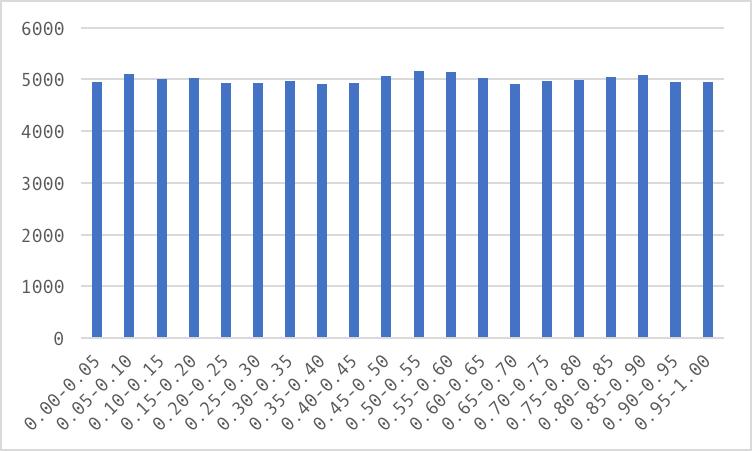
\includegraphics[width=0.5\textwidth]{100000a.png}}
    \caption{Histograms for $a = 16807$, $m = 2^{31} - 1$, and $x_{0} = 1$ :\\(a) n = 1000, (b) n = 10000 and (c) n = 100000}
\end{figure}

\begin{figure}[H]
  \centering
  \captionsetup{justification=centering}
  \subfloat[$\xi_{1}$]{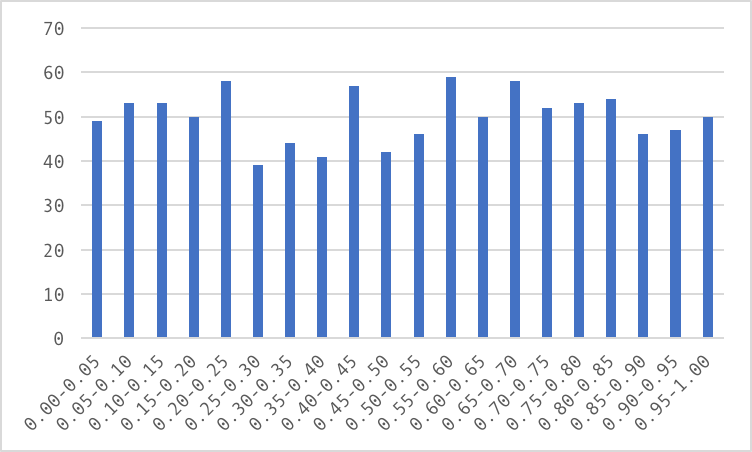
\includegraphics[width=0.5\textwidth]{1000b.png}}\hspace{10mm}
  \subfloat[$\xi_{2}$]{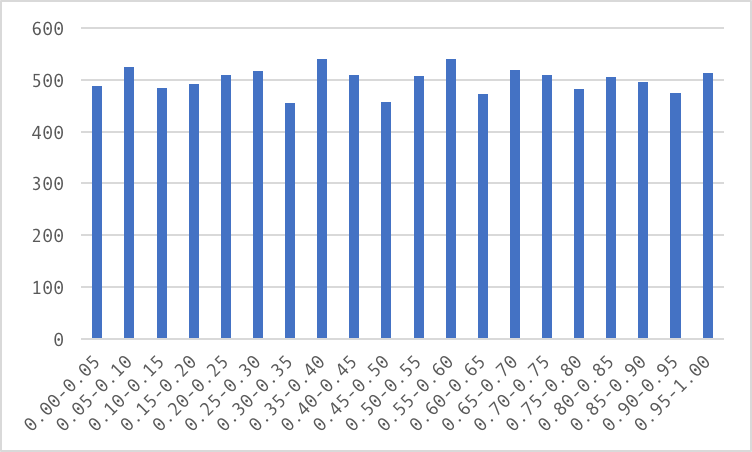
\includegraphics[width=0.5\textwidth]{10000b.png}}\\
  \subfloat[$\xi_{3}$]{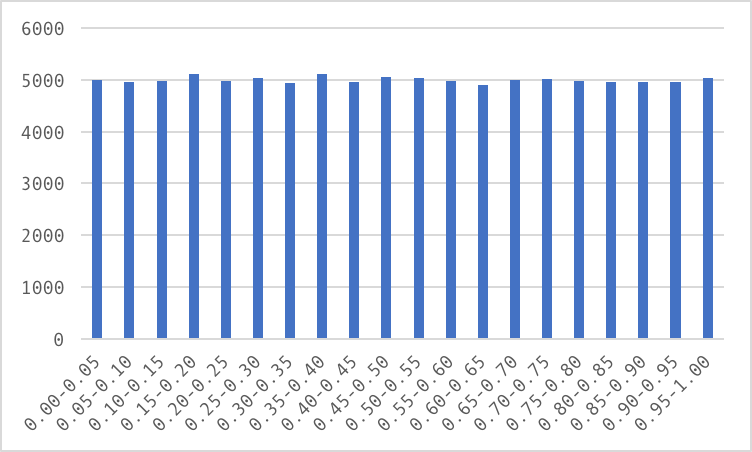
\includegraphics[width=0.5\textwidth]{100000b.png}}
    \caption{Histograms for $a = 40692$, $m = 214748339$, and $x_{0} = 1$ :\\(a) n = 1000, (b) n = 10000 and (c) n = 100000}
\end{figure}

\begin{figure}[H]
  \centering
  \captionsetup{justification=centering}
  \subfloat[$\xi_{1}$]{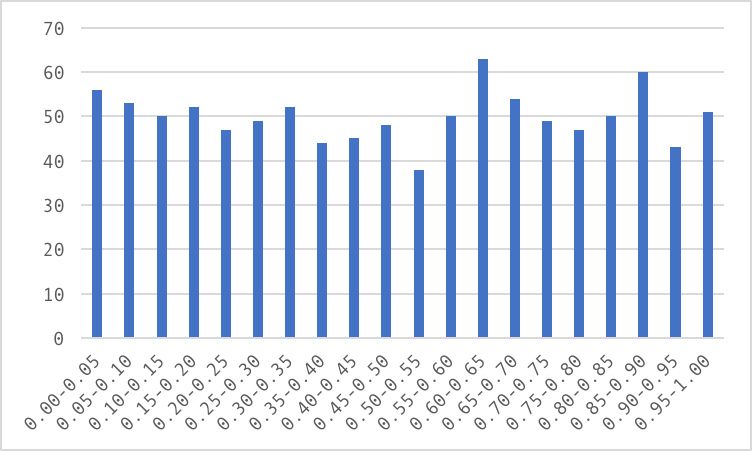
\includegraphics[width=0.5\textwidth]{1000c.png}}\hspace{10mm}
  \subfloat[$\xi_{2}$]{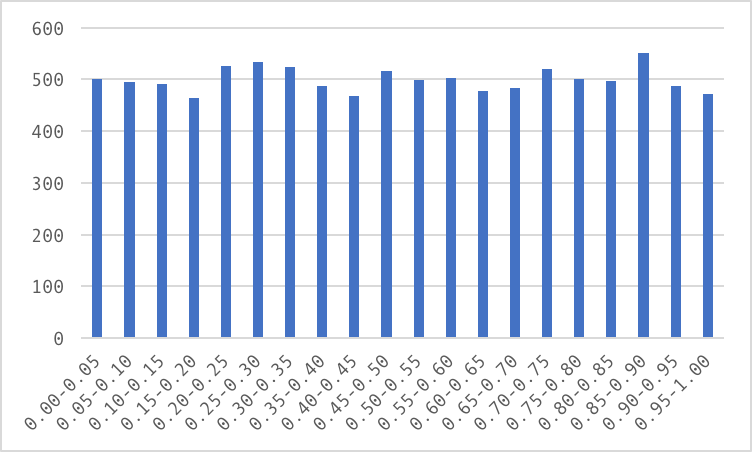
\includegraphics[width=0.5\textwidth]{10000c.png}}\\
  \subfloat[$\xi_{3}$]{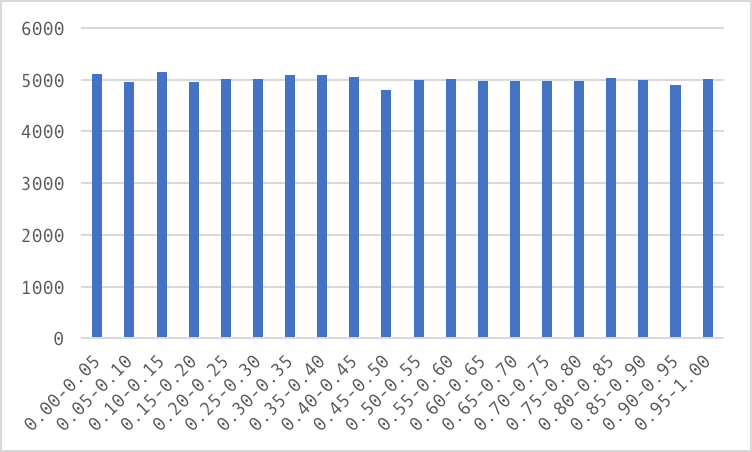
\includegraphics[width=0.5\textwidth]{100000c.png}}
    \caption{Histograms for $a = 40014$, $m = 214748356$, and $x_{0} = 1$ :\\(a) n = 1000, (b) n = 10000 and (c) n = 100000}
\end{figure}

The picture shows that the generated numbers are correct, since on increasing n we are getting the proper shape of uniform distribution.
\newpage
For $n = 100000$, $a = 16807$, $m = 2^{31} - 1$, and $x_{0} = 1$, the plot $(u_i, u_{i+1})$ is as follows :

\begin{figure}[H]
  \centering
  \subfloat[$\xi_{1}$]{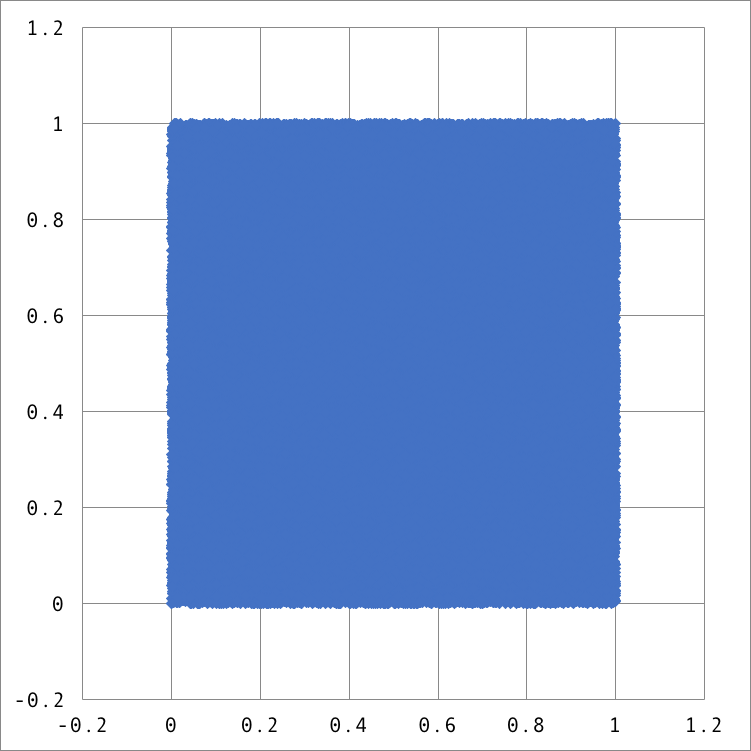
\includegraphics[width=0.5\textwidth]{plot.png}}
      \caption{Plot $(u_i, u_{i+1})$}
\end{figure}

\begin{figure}[H]
  \centering
  \subfloat[$\xi_{1}$]{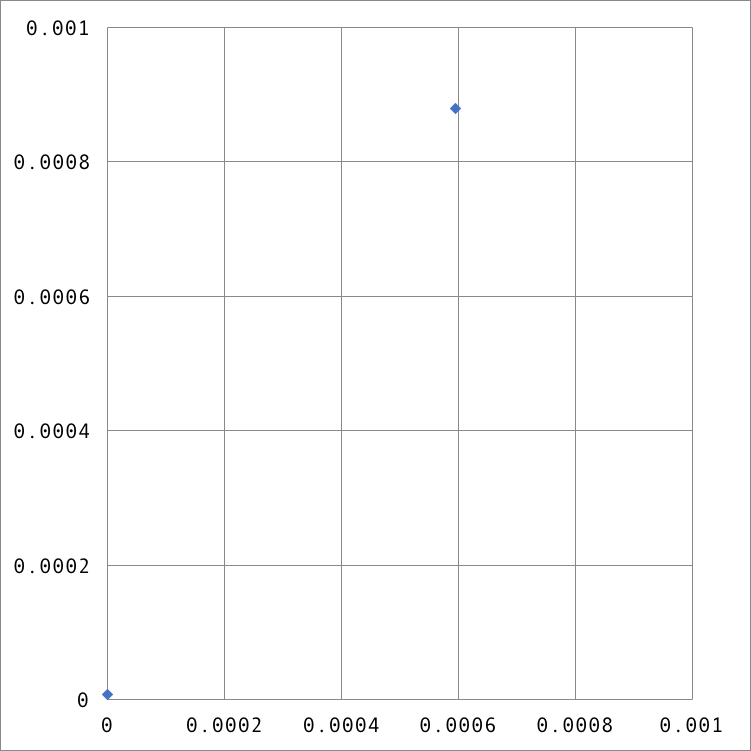
\includegraphics[width=0.5\textwidth]{zoom.png}}
      \caption{Plot $(u_i, u_{i+1})$ zoomed into the range $u_i$ $\epsilon$ [0, 0.001]}
\end{figure}

The picture shows that the numbers generated are truly i.i.d. Uniform(0,1), as we see points randomly dispersed in the unit square, in the plot of the sequence $(u_{i-1}, u{i})$.\\
On zooming into the given interval [0, 0.001], we observe that the density of numbers generated is low and distinctively spaced, and the dispersion is not thorough enough.\\
Although on increasing the number of values generated, the random dispersion will be more efficient, since, the density of the random numbers generated will increase.\\\\
Hence, it is concluded that the given random value generator is efficient.

\newpage

\begin{enumerate}
\item[Q 2] Consider the extended Fibonacci generator :
$U_i = (U_{i-17} + U_{i-5}) ~~ \mbox{mod} ~~ 2^{31}$.

(a) Use the linear congruence generator to generate the first 17 values of $U_i$.
(b) Then generate the values of $U_i$ (say for 1000, 10000 and 100000 values).
(c) For each of the above set of values plot $(U_{i}, U_{i+1})$.
(d) Observe (give the values) the convergence of the sample mean and sample variance towards actual values, and generate a probability distribution with, say, 1000 values generated.
(e) Compute the autocorrelation of lags 1, 2, 3, 4, and 5 with 1000 generated values.
\end{enumerate}

\noindent{Code for C}

\begin{lstlisting}
#include <stdio.h>
#include <stdlib.h>
#include <math.h>

void list(int v0, float * u){
  long long int x[v0]; int v = 0;
  x[0] = 1;
	u[0] = (x[0]/(float)pow(2,31));
//LCG
	while(v < 17 && v < v0){
    v++;
		x[v] = (((16807 * x[v-1]) + 0) % (long long int)(pow(2,31) - 1));
		u[v] = (x[v]/(float)(pow(2,31) - 1));
  }
//Extended Fibonacci Generator
  while(v < v0){
    v++;
		x[v] = ((x[v-17] + x[v-5]) % (long long int)pow(2,31));
    u[v] = (x[v]/(float)pow(2,31));
	}
  
}

void data(float * u, int n){
  for (int i = 1; i < n; i++) {
    printf("(%g,%g)\t", u[i-1], u[i]);
  }
}

float mean(float * u, int n){
  float m = 0;
  for (int i = 0; i < n; i++) {
    m += (u[i]/(float)n);
  }
  return m;
}

float variance(float * u, int n, float mu){
  float v = 0;
  for (int i = 0; i < n; i++) {
    v += (pow((u[i]- mu),2)/(float)n);
  }
  return v;
}

float rho(float * u, int n, int l, float mu){
  float num = 0, denom = 0;

  for (int t = l+1; t <= n; t++) {
    num += ((u[t] - mu) * (u[t - l] - mu));
  }

  for (int t = 1; t <= n; t++) {
    denom += pow((u[t]- mu),2);
  }

  return (num / denom);
}

void main(){
  float u[1000000];
  list(100000, u);
  
  printf("Plot data :");
  printf("\n\t#For 1000 values ::\n");
  data(u, 1000);

  printf("\n\t#For 10000 values ::\n");
  data(u, 10000);

  printf("\n\t#For 100000 values ::\n");
  data(u, 100000);
  printf("\n");

  float mu = mean(u, 1000);
  printf("\nThe sample mean for 1000 values is %g.\n", mu);

  float var = variance(u, 1000, mu);
  printf("\nThe sample variance for 1000 values is %g.\n\n", var);

//Autocorrelation of lags
  for (int i = 1; i <= 5; i++) {
    printf("Autocorrelation of lag %d, with 1000 generated values, is %g.\n", i, rho(u, 1000, i, mu));
  }
}
\end{lstlisting}
\newpage
\noindent{\textbf{Result}:}

The plots $(u_i , u_{i+1})$ can be shown as :

\begin{figure}[H]
  \centering
  \subfloat[$\xi_{1}$]{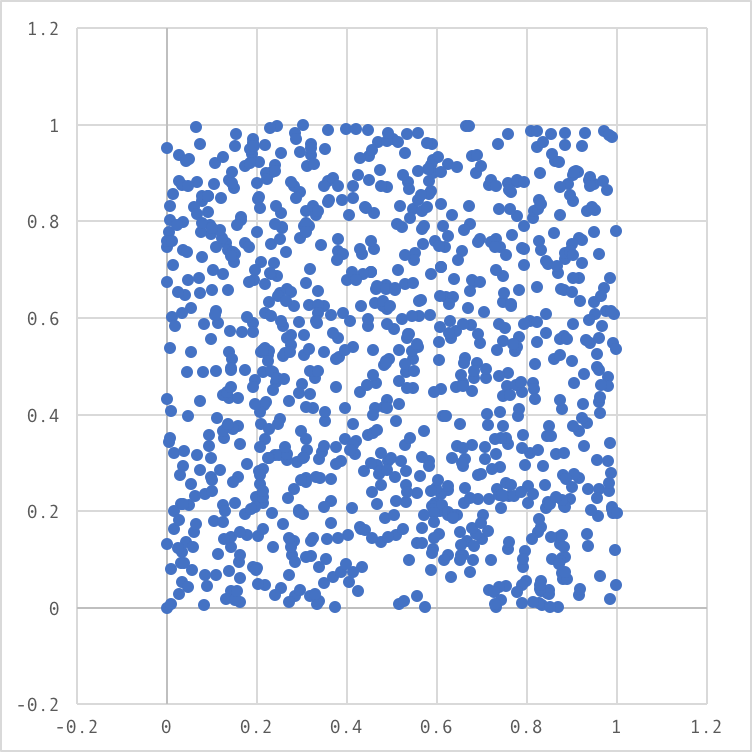
\includegraphics[width=0.45\textwidth]{plot1000.png}}\hspace{10mm}
  \subfloat[$\xi_{2}$]{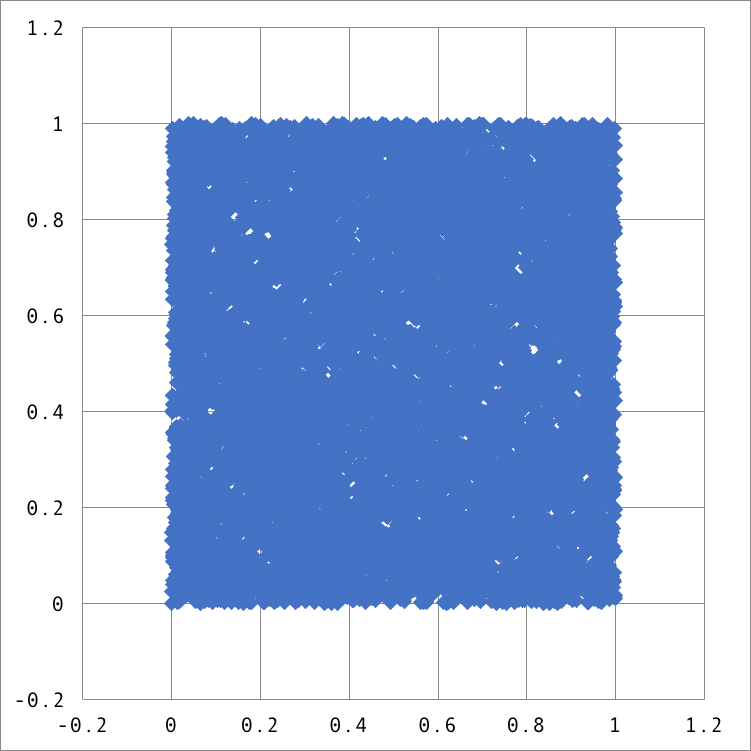
\includegraphics[width=0.45\textwidth]{plot10000.png}}\\
  \subfloat[$\xi_{3}$]{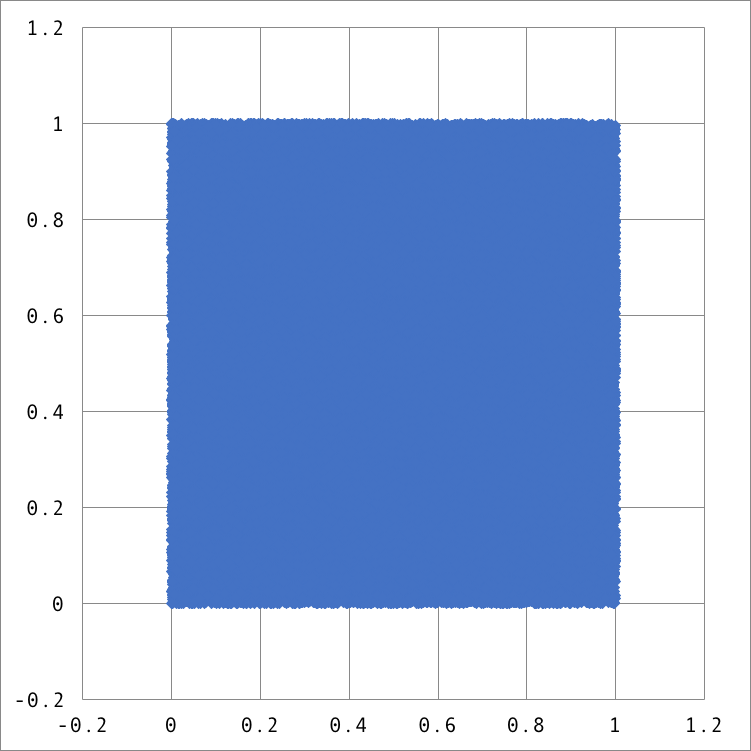
\includegraphics[width=0.45\textwidth]{plot100000.png}}
    \caption{Plot $(u_i , u_{i+1})$ for (a) n = 1000, (b) n = 10000 and (c) n = 100000}
\end{figure}

The sample mean and sample variance, calculated for 1000 values, are 0.493665 and 0.0827854 respectively, which are close to theoretical mean $\frac{1}{2}$ i.e. 0.5 and theoretical variance $\frac{1}{12}$ i.e. 0.0833333.

Autocorrelation of lag 1, with 1000 generated values, is -0.0355444.\\
Autocorrelation of lag 2, with 1000 generated values, is -0.0508289.\\
Autocorrelation of lag 3, with 1000 generated values, is -0.0167786.\\
Autocorrelation of lag 4, with 1000 generated values, is 0.0189976.\\
Autocorrelation of lag 5, with 1000 generated values, is -0.0254554.

\end{document}